\documentclass[journal,12pt,twocolumn]{IEEEtran}
%
\usepackage{setspace}
\usepackage{gensymb}
\usepackage{xcolor}
\usepackage{caption}
%\usepackage{subcaption}
%\doublespacing
\singlespacing
\usepackage{multicol}
%\usepackage{eenrc}
%\usepackage{iithtlc}
%\usepackage{graphicx}
%\usepackage{amssymb}
%\usepackage{relsize}
\usepackage[cmex10]{amsmath}
\usepackage{mathtools}
%\usepackage{amsthm}
%\interdisplaylinepenalty=2500
%\savesymbol{iint}
%\usepackage{txfonts}
%\restoresymbol{TXF}{iint}
%\usepackage{wasysym}
\usepackage{amsthm}
\usepackage{mathrsfs}
\usepackage{txfonts}
\usepackage{stfloats}
\usepackage{cite}
\usepackage{cases}
\usepackage{subfig}
%\usepackage{xtab}
\usepackage{longtable}
\usepackage{multirow}
%\usepackage{GPIO 0 pinalgorithm}
%\usepackage{algpseudocode}
\usepackage{enumitem}
\usepackage{mathtools}
%\usepackage{stmaryrd}
\usepackage{graphicx}
\usepackage{listings}
\usepackage{circuitikz}
    \usepackage[latin1]{inputenc}                                 %%
    \usepackage{color}                                            %%
    \usepackage{array}                                            %%
    \usepackage{longtable}                                        %%
    \usepackage{calc}                                             %%
    \usepackage{multirow}                                         %%
    \usepackage{hhline}                                           %%
    \usepackage{ifthen}                                           %%
  %optionally (for landscape tables embedded in another document): %%
    \usepackage{lscape}     
\usepackage{url}
\def\UrlBreaks{\do\/\do-}

%\usepackage{wasysym}
%\newcounter{MYtempeqncnt}
\DeclareMathOperator*{\Res}{Res}
%\renewcommand{\baselinestretch}{2}
\renewcommand\thesection{\arabic{section}}
\renewcommand\thesubsection{\thesection.\arabic{subsection}}
\renewcommand\thesubsubsection{\thesubsection.\arabic{subsubsection}}

\renewcommand\thesectiondis{\arabic{section}}
\renewcommand\thesubsectiondis{\thesectiondis.\arabic{subsection}}
\renewcommand\thesubsubsectiondis{\thesubsectiondis.\arabic{subsubsection}}

% correct bad hyphenation here
\hyphenation{op-tical net-works semi-conduc-tor}

\def\inputGnumericTable{}  

\lstset{
language=python,
frame=single, 
breaklines=true
}

\begin{document}
%

\theoremstyle{definition}

\newtheorem{theorem}{Theorem}[section]
\newtheorem{problem}{Problem}
\newtheorem{proposition}{Proposition}[section]
\newtheorem{lemma}{Lemma}[section]
\newtheorem{corollary}[theorem]{Corollary}
\newtheorem{example}{Example}[section]
\newtheorem{definition}{Definition}[section]
%\newtheorem{algorithm}{Algorithm}[section]
%\newtheorem{cor}{Corollary}
\newcommand{\BEQA}{\begin{eqnarray}}
\newcommand{\EEQA}{\end{eqnarray}}
\newcommand{\define}{\stackrel{\triangle}{=}}

\bibliographystyle{IEEEtran}
%\bibliographystyle{ieeetr}



\providecommand{\pr}[1]{\ensuremath{\Pr\left(#1\right)}}
\providecommand{\qfunc}[1]{\ensuremath{Q\left(#1\right)}}
\providecommand{\sbrak}[1]{\ensuremath{{}\left[#1\right]}}
\providecommand{\lsbrak}[1]{\ensuremath{{}\left[#1\right.}}
\providecommand{\rsbrak}[1]{\ensuremath{{}\left.#1\right]}}
\providecommand{\brak}[1]{\ensuremath{\left(#1\right)}}
\providecommand{\lbrak}[1]{\ensuremath{\left(#1\right.}}
\providecommand{\rbrak}[1]{\ensuremath{\left.#1\right)}}
\providecommand{\cbrak}[1]{\ensuremath{\left\{#1\right\}}}
\providecommand{\lcbrak}[1]{\ensuremath{\left\{#1\right.}}
\providecommand{\rcbrak}[1]{\ensuremath{\left.#1\right\}}}
\theoremstyle{remark}
\newtheorem{rem}{Remark}
\newcommand{\sgn}{\mathop{\mathrm{sgn}}}
\providecommand{\abs}[1]{\left\vert#1\right\vert}
\providecommand{\res}[1]{\Res\displaylimits_{#1}} 
\providecommand{\norm}[1]{\lVert#1\rVert}
\providecommand{\mtx}[1]{\mathbf{#1}}
\providecommand{\mean}[1]{E\left[ #1 \right]}
\providecommand{\fourier}{\overset{\mathcal{F}}{ \rightleftharpoons}}
%\providecommand{\hilbert}{\overset{\mathcal{H}}{ \rightleftharpoons}}
\providecommand{\system}{\overset{\mathcal{H}}{ \longleftrightarrow}}
\providecommand{\gauss}[2]{\mathcal{N}\ensuremath{\left(#1,#2\right)}}
	%\newcommand{\solution}[2]{\textbf{Solution:}{#1}}
\newcommand{\solution}{\noindent \textbf{Solution: }}
\providecommand{\dec}[2]{\ensuremath{\overset{#1}{\underset{#2}{\gtrless}}}}
%\numberwithin{equation}{section}
%\numberwithin{problem}{section}

\def\putbox#1#2#3{\makebox[0in][l]{\makebox[#1][l]{}\raisebox{\baselineskip}[0in][0in]{\raisebox{#2}[0in][0in]{#3}}}}
     \def\rightbox#1{\makebox[0in][r]{#1}}
     \def\centbox#1{\makebox[0in]{#1}}
     \def\topbox#1{\raisebox{-\baselineskip}[0in][0in]{#1}}
     \def\midbox#1{\raisebox{-0.5\baselineskip}[0in][0in]{#1}}


% paper title
% can use linebreaks \\ within to get better formatting as desired

%\title{FM SiGPIO 0 pingnal Transmission Using Pi}
 
 
%\title{Electrical Circuit Design using Latex}

%\title{\logo{C \& Python Programming using Termux}}
\title{Controlling of LED using ESP8266 WiFi module}


\author{N Jagadeeswar$^{1}$, Gautam Kumar$^{2}$,and G V V Sharma$^{*}$ %<-this  stops a space
\thanks{The authors were interns of Summer Internship Program 2019  of IITH under Dr.G.V.V.Sharma with the Department
of Electrical Engineering, Indian Institute of Technology, Hyderabad 502285 India  Email:  naramalajagadeeswar@gmail.com$^{1}$, eid4gautam@gmail.com$^{2}$, gadepall@iith.ac.in$^{*}$}}


% make the title area
\maketitle


\tableofcontents

\bigskip

\begin{abstract}
This manual pinovides an introduction to ESP8266 wifi module. This WiFi module acts as a station mode, Access point mode and both at  a time.
\end{abstract}
\begin{figure}[h!]
\centering
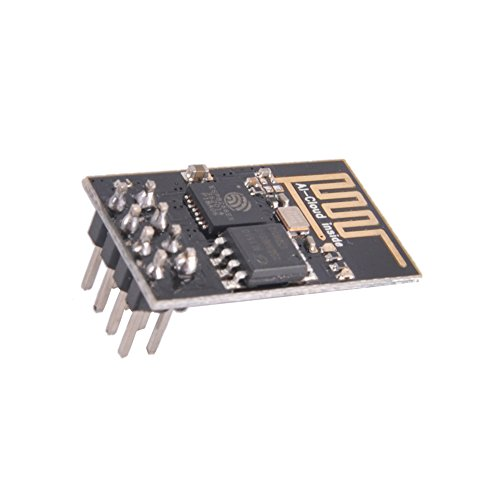
\includegraphics[height = 5cm, width = 5cm]{images/esp8266.jpeg}
\caption{ESP8266 Module}
\end{figure}
\begin{itemize}
\item The ESP8266 module consists of 8 pins which are arranged in 4x2 order. The labeling of these pins are as shown in below table
\end{itemize}
\section{ESP8266}
\begin{center}
\begin{tabular}{ |c|c| } 
\hline
TX    & GND       \\
\hline
CH_PD & GPIO 2    \\
\hline
RST   & GPIO 0    \\
\hline
Vcc   & RX        \\
\hline
\end{tabular}
\end{center}

\section{CONNECTIONS WITH ARDUINO}
\begin{center}
\begin{tabular}{ |c|c| } 
\hline
Arduino & ESP8266       \\
\hline
Vcc & Vcc \& CH-PD    \\
\hline
GND   & GPIO 0 \& GND   \\
\hline
TX  & TX        \\
\hline
RX  & RX    \\
\hline
\end{tabular}
\end{center}
\begin{itemize}
\item Remove the ATMEGA328 chip from Arduino before uploading the program.
\item Connect the GPIO 0 pin to GND during flashing the code and remove the GPIO 0 pin after flashing. We can use GPIO 2 pin for LED.
\item Use 3.3 volts for Vcc
\end{itemize}
\section{INSTRUCTIONS BEFORE UPLOADING THE PROGRAM}
\begin{itemize}
\item Open Arduino IDE software.
\item Go to File, At the bottom you will find preferences. Paste the following link and then click on OK.link 
\url{http://arduino.esp8266.com/stable/package_esp8266com_index.json}
\item Go to the the tools click on Board at the top you will find Board manager click on it.
\item In Board manager you will find lot of Boards but we have to install ESP8266 Board. Search for ESP8266 and install it.
\item After installing the ESP8266 Board , Go to tools again and click on Board select the 'Generic ESP8266 Module' Board.
\item Since we have to upload the program into the the ESP8266 Board we installed the ESP8266 Board. Here we use Arduino for power supply ,TX and RX pins. We will not use any Digital pins.
\item After completion of all above settings upload the following code into the Arduino.
\item Before uploading the code Add the required libraries mentioned in the program. 
\end{itemize}

\section{PROGRAM}
\lstinputlisting[language=c]{codes/LED_BLINK.ino}
\begin{itemize}
\item Before uploading the program give your mobile hotspot NAME and PASSWORD. In this program i have given 'motorola' as hotspot name password as 'gautam1234'.
\item After uploading the program remove GPIO 0 from GND.
\item check serial moniter you will find "connecting............." . After conncting serial moniter will display 
"mDNS responder started"
"HTTP server started"
and WiFi IP Address will display like "192.168.43.161".
\item Paste the generated IP in your browser and browse you will find "Toggle LED" on the browser.
\item click on "Toggle LED" to ON and OFF the LED.
\end{itemize}
\begin{thebibliography}{00}
\bibitem{b1} program \url{https://tttapa.github.io/ESP8266/Chap10%20-%20Simple%20Web%20Server.html}.
\end{thebibliography}
\end{document}
